\documentclass[border=6pt]{standalone}
\usepackage{ctex,amsmath,amssymb,tikz}
\usetikzlibrary{arrows.meta,positioning,patterns,calc,decorations.pathreplacing}
\begin{document}
% 圆锥 z^2=(h^2/R^2)(x^2+y^2) 的上半部。
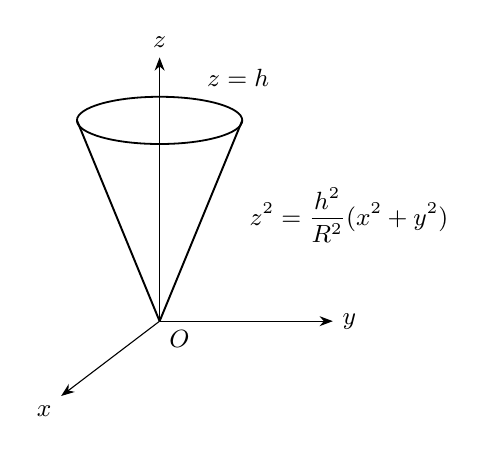
\begin{tikzpicture}[>=Stealth,font=\small,line join=round]
  \draw[->] (0,0) -- (2.2,0) node[right] {$y$};
  \draw[->] (0,0) -- (-1.25,-.95) node[below left] {$x$};
  \draw[->] (0,0) -- (0,3.35) node[above] {$z$};
  \draw[line width=.7pt] (0,0) -- (-1.05,2.55);
  \draw[line width=.7pt] (0,0) -- (1.05,2.55);
  \draw[line width=.65pt] (0,2.55) ellipse[x radius=1.05,y radius=.3];
  \node[below right] at (0,0) {$O$};
  \node[above right] at (.48,2.85) {$z=h$};
  \node[right,align=left] at (1.02,1.35)
    {$\displaystyle z^2=\frac{h^2}{R^2}(x^2+y^2)$};
\end{tikzpicture}

\end{document}